\documentclass[12pt]{article}
\newif\ifshowsolutions
\showsolutionsfalse
%\showsolutionstrue

%% arXiv paper template by Flip Tanedo
%% last updated: Dec 2016



%%%%%%%%%%%%%%%%%%%%%%%%%%%%%
%%%  THE USUAL PACKAGES  %%%%
%%%%%%%%%%%%%%%%%%%%%%%%%%%%%

\usepackage{amsmath}
\usepackage{amssymb}
\usepackage{amsfonts}
\usepackage{graphicx}
\usepackage{xcolor}
\usepackage{nopageno}
\usepackage{enumerate}
\usepackage{parskip}
\usepackage{comment}
	
	
%http://tex.stackexchange.com/questions/15509/hide-custom-environment-content-based-on-boolean
\ifshowsolutions
	\newenvironment{solution}%
	{\color{blue!60!black}
	\textsf{\textbf{Solution}}:
	}%
	%
	{\ignorespacesafterend}
\else
	\excludecomment{solution}
\fi
	
%\newenvironment{solution}
%    {%\begin{sol}
%    \textcolor{blue!40!black}{
%	\textbf{Solution}:}
%    }
%    { 
%    %\end{sol}
%    }
%    
%%\includecomment{solution}




%%%%%%%%%%%%%%%%%%%%%%%%%%%%%%%%%
%%%  UNUSUAL PACKAGES        %%%%
%%%  Uncomment as necessary. %%%%
%%%%%%%%%%%%%%%%%%%%%%%%%%%%%%%%%

\usepackage{titlesec}
\titleformat*{\section}{\large\bfseries}

%% MATH AND PHYSICS SYMBOLS
%% ------------------------
%\usepackage{slashed}       % \slashed{k}
%\usepackage{mathrsfs}      % Weinberg-esque letters
%\usepackage{youngtab}	    % Young Tableaux
%\usepackage{pifont}        % check marks
\usepackage{bbm}           % \mathbbm{1} incomp. w/ XeLaTeX 
%\usepackage[normalem]{ulem} % for \sout


%% CONTENT FORMAT AND DESIGN (below for general formatting)
%% --------------------------------------------------------
\usepackage{lipsum}        % block of text (formatting test)
%\usepackage{color}         % \color{...}, colored text
%\usepackage{framed}        % boxed remarks
%\usepackage{subcaption}    % subfigures; subfig depreciated
%\usepackage{paralist}      % compactitem
%\usepackage{appendix}      % subappendices
%\usepackage{cite}          % group cites (conflict: collref)
%\usepackage{tocloft}       % Table of Contents	


%% TABLES IN LaTeX
%% ---------------
%\usepackage{booktabs}      % professional tables
%\usepackage{nicefrac}      % fractions in tables,
%\usepackage{multirow}      % multirow elements in a table
%\usepackage{arydshln} 	    % dashed lines in arrays

%% Other Packages and Notes
%% ------------------------
%\usepackage[font=small]{caption} % caption font is small



%\renewcommand{\thesection}{}
%\renewcommand{\thesubsection}{\arabic{subsection}}

%%%%%%%%%%%%%%%%%%%%%%%%%%%%%%%%%%%%%%%%%%%%%%%
%%%  PAGE FORMATTING and (RE)NEW COMMANDS  %%%%
%%%%%%%%%%%%%%%%%%%%%%%%%%%%%%%%%%%%%%%%%%%%%%%

\usepackage[margin=2cm]{geometry}   % reasonable margins

\graphicspath{{figures/}}	        % set directory for figures

% for capitalized things
\newcommand{\acro}[1]{\textsc{\MakeLowercase{#1}}}    

\numberwithin{equation}{section}    % set equation numbering
\renewcommand{\tilde}{\widetilde}   % tilde over characters
\renewcommand{\vec}[1]{\mathbf{#1}} % vectors are boldface

\newcommand{\dbar}{d\mkern-6mu\mathchar'26}    % for d/2pi
\newcommand{\ket}[1]{\left|#1\right\rangle}    % <#1|
\newcommand{\bra}[1]{\left\langle#1\right|}    % |#1>
\newcommand{\Xmark}{\text{\sffamily X}}        % cross out

% Change list spacing (instead of package paralist)
% from: http://en.wikibooks.org/wiki/LaTeX/List_Structures#Line_spacing
%\let\oldenumerate\enumerate
%\renewcommand{\enumerate}{
%  \oldenumerate
%  \setlength{\itemsep}{1pt}
%  \setlength{\parskip}{0pt}
%  \setlength{\parsep}{0pt}
%}

\let\olditemize\itemize
\renewcommand{\itemize}{
  \olditemize
  \setlength{\itemsep}{1pt}
  \setlength{\parskip}{0pt}
  \setlength{\parsep}{0pt}
}


% Commands for temporary comments
\newcommand{\flip}[1]{{\color{red} [\textbf{Flip}: {#1}]}}
\newcommand{\email}[1]{\texttt{\href{mailto:#1}{#1}}}

\newenvironment{institutions}[1][2em]{\begin{list}{}{\setlength\leftmargin{#1}\setlength\rightmargin{#1}}\item[]}{\end{list}}


\usepackage{fancyhdr}		% to put preprint number



% Commands for listings package
%\usepackage{listings}      % \begin{lstlisting}, for code
%
% \lstset{basicstyle=\ttfamily\footnotesize,breaklines=true}
%    sets style to small true-type


%%%%%%%%%%%%%%%%%%%%%%%%%%%%%%%%%%%%%%%%%%%%%%
%%%  TIKZ COMMANDS FOR EXTERNAL DIAGRAMS  %%%%
%%%  requires -shell-escape               %%%%
%%%  in texpad 1.7: prefs > shell esc sec %%%%
%%%%%%%%%%%%%%%%%%%%%%%%%%%%%%%%%%%%%%%%%%%%%%

%% This is for exporting tikz figures as into a ./tikz/ subfolder.
%% It is useful if you want pdf versions of the tikz diagrams or
%% if you need to speed up compilation of a large document with
%% many tikz diagrams.

%\write18{} % Careful with this!
%\usetikzlibrary{external}
%\tikzexternalize[prefix=tikz/] % folder for external pdfs


%%%%%%%%%%%%%%%%%%%
%%%  HYPERREF  %%%%
%%%%%%%%%%%%%%%%%%%

%% This package has to be at the end; can lead to conflicts
\usepackage{microtype}
\usepackage[
	colorlinks=true,
	citecolor=black,
	linkcolor=black,
	urlcolor=green!50!black,
	hypertexnames=false]{hyperref}



%%%%%%%%%%%%%%%%%%%%%
%%%  TITLE DATA  %%%%
%%%%%%%%%%%%%%%%%%%%%

%%% PREPRINT NUMBER USING fancyhdr
%%% Don't forget to set \thispagestyle{firststyle}
%%% ----------------------------------------------
%\renewcommand{\headrulewidth}{0pt} % no separator
%\fancypagestyle{firststyle}{
%\rhead{\footnotesize \texttt{UCI-TR-2016-XX}}}

\renewcommand{\thesubsection}{\thesection.\alph{subsection}}

\begin{document}

%\thispagestyle{empty}
%\thispagestyle{firststyle} %% to include preprint

\begin{center}

    {\Large \textsc{Homework 6:} 
    \textbf{Maximal Extensions, Conformal Diagrams}}


    
\end{center}

\vskip .4cm

\noindent
\begin{tabular*}{\textwidth}{rlcrll}
	\textsc{Course:}& Physics 208, {General Relativity} (Winter 2017)
	&
%	\hspace{1.2cm}
	&
	\\
	\textsc{Instructor:}& Flip Tanedo (\email{flip.tanedo@ucr.edu})
	&
	%\hfill
	&
	& 
	\\
	\textsc{Due Date:}& \textbf{Thursday, March 2} in class. (No class on Tuesday, Feb 28.)
	&
	%\hfill
	&
	%	
\end{tabular*}

You are required to complete the {\textsf{Reading Assignment}} and {\textsf{Essential Problems}} below. 
%
Please let me know if these are too time intensive. %\footnote{The `essential problems' are meant to be a bare minimum of independent work to follow the course.}.
%
You are invited to explore the `extra' problems as they apply to your goals for this course: {\textsf{Mathematical Problems}} develop geometric intuition, while {\textsf{Phenomenological Problems}} are applications of relativity. 
% 



\vspace{2em}
{\Large\textbf{\textsf{Reading Assignment}}}

Read the following topics. You may choose to read the analogous topics in an appropriate textbook or reference of your preference. Most of this reading is meant to be complementary to the approach in the lectures.

\begin{itemize}
%	\item Finish chapter 12 of Hartle
%	\item We will not spend much time on more realistic black holes, but feel free to peruse chapters 13 -- 15 as you are interested. For an excellent set of lecture notes, see \texttt{gr-qc/9707012}.
%	\item You can start reading chapter 18 on cosmological models---we will not discuss them too much in class, but we will play with FRW metrics in upcoming homework. 
	\item Finish reading about the Einstein equation, chapter 21 of Hartle.
\end{itemize}

\vspace{2em}

The Schwarzchild metric is:
\begin{align}
	ds^2 = \left(1-\frac{r_s}{r}\right)dt^2 
	- \left(1-\frac{r_s}{r}\right)^{-1}dr^2
	- r^2 d\Omega^2 \ .
\end{align}
We've written $r_s = 2GM$ as the Schwarzschild radius.


\textsc{Caveat emptor}: as always, do what I mean, not necessarily what I say.


\vspace{2em}
{\Large\textbf{\textsf{Essential Problems}}}

\section{Rindler Space}

% Wald, 6.4

Rindler spacetime is a nice 2D analog to Schwarzschild spacetime,
\begin{align}
	ds^2 = x^2 dt^2 - dx^2 \ .
	\label{eq:original:Rindler}
\end{align}
We restrict the coordinates to $-\infty < t < \infty$ and $0 \leq x < \infty$. 
\begin{enumerate}[(a)]
	\item Calculate the Ricci scalar at $x=0$ to identify that nothing bad happens there. We now suspect that the apparent singularity there ($g = 0$) may only be a coordinate singularity.
	\item What are the null geodesics of Rindler space? Draw a few of them.
	\item Define null coordinates $u$ (the one with a relative minus sign) and $v$ (the one with a relative plus sign) so that $u=$constant and $v=$constant correspond to null geodesics. Show that the metric in terms of $u$ and $v$ is
	\begin{align}
		ds^2 = e^{v-u}dv\,du \ .
	\end{align}
	\item Observe that the $(u,v)$ coordinates are defined for $-\infty < u,v < \infty$, but that these still correspond go $x\geq 0$. 
	
		Analogously to what we did in class for Kruskal coordinates, we may define coordinates that extend this space. In other words, we may `pull the $x=0$ point' back into the space. Based on the form of the metric, guess what these coordinates $\tilde u$ and $\tilde v$ might be.
		
	\item To derive $\tilde u$ and $\tilde v$ more systematically, note that the original metric (\ref{eq:original:Rindler}) has a time-like Killing vector, $K_{(t)} = \partial/\partial t = (1,0)$. The conserved quantity is the energy, $E = g_{\mu\nu} K_{(t)}^\mu \dot x^\nu$; write this explicitly in terms of $dt/d\lambda$, where $\lambda$ is the affine parameter of a geodesic.
	\item For an \emph{outgoing} null geodesic (constant $u$) integrate the expression in part (e) in the $(u,v)$ coordinates. Show that:
	\begin{align}
		\lambda = \frac{e^{v-u}}{2E} + \text{constant} \ .
	\end{align}
 	Recalling that $u$ is constant on these outgoing null geodesic, this tells us that we may choose choose $\lambda_\text{out} = e^{v}$ as an affine parameter for an outgoing null geodesic. Similarly, $\lambda_\text{in} = -e^{-u}$ is a good parameter for in-going null geodesics.  The affine parameters have limited ranges, which is a hint that the geodesics of (\ref{eq:original:Rindler}) are incomplete.
 	\item Perform a coordinate transformation
 	\begin{align}
 		\tilde u &= -e^{-u} 
 		&
 		\tilde v &= e^{v}
 	\end{align}
	and write the metric in a very simple form. Observe that the spacetime is well defined for $-\infty < \tilde u, \tilde v < \infty$. What sub-region of this corresponds to the original Rindler spacetime?
	\item Finally, convert from null coordinates back to space and time coordinates
	\begin{align}
		X &= \frac 12 \left( \tilde v -\tilde u\right)
		&
		T &= \frac 12 \left( \tilde v +\tilde u\right) \ .
	\end{align}
	Write the metric in $(X,T)$ coordinates. You should rediscover something familiar---revel in this M.\ Night Shyamalan moment.
\end{enumerate}

\vspace{2em}
{\Large\textbf{\textsf{Phenomenological Problems}}}

\section{Timing your fall into a black hole.} \textsc{Hartle problem 12-5}. An observer falls radially into a spherical black hole of mass $M$. The observer starts from rest relative to a stationary observer at a Schwarzschild coordinate radius of $10GM = 5r_s$ how much time elapses on the observer's own clock before hitting the singularity?




\vspace{2em}
{\Large\textbf{\textsf{Mathematical Problems}}}


\section{Conformal Diagram of Minkowski Space}

Conformal (Penrose) diagrams are a visual language for representing a spacetime. We will follow the general steps that we took for the Schwarzschild black hole. Starting from ordinary Minkowski space,
\begin{align}
	ds^2 = dt^2 - dr^2 - r^2 d\Omega^2 \ ,
\end{align}
let us derive the conformal diagram through the following steps.
\begin{enumerate}[(a)]
\item Convert to null coordinates,
\begin{align}
	u & = t-r
	&
	v &= t+r \ .
\end{align}	
Write the metric in these coordinates. What are the ranges of these variables?
\item We want to bring $\infty$ to finite regions of our space, so define $(U,V)$ coordinates by
\begin{align}
	\tan U &= u 
	&
	\tan V &= v \ .
\end{align}
A good choice of range is $-\pi/2 < U,V < \pi/2$. What additional condition is there on $U$ and $V$? \textsc{Hint}: $r\geq 0$. Write the metric in $(U,V)$ coordinates. Recall that $d\tan x = dx/\cos^2 x$. You may also use:
\begin{align}
	\left(\tan x - \tan y\right)^2
	&= \frac{\sin^2(x-y)}{\cos^2x \cos^2y}
\end{align} \ .
\item Now that we are armed with null coordinates that only span a finite range, we may convert back into a natural time and space coordinate via
\begin{align}
	T&= V+U & R&=V-U \ .
\end{align}
Write the metric in these coordinates, the range of coordinates, and any additional constraints on $T$ and $R$. Observe that the metric takes the form:
\begin{align}
	ds^2 = \omega^{-2}(T,R) \left[dT^2 - dR^2 - \sin^2 R \, d\Omega^2 \right] \ .
	\label{eq:mink:conf:flat}
\end{align}
Write out what $\omega$ is. Observe that $\omega^{-2}$ is an overall multiplicative factor on the spacetime, and further than null geodesics have $45^\circ$ trajectories.
\item As an aside: write down the metric for a 4D cylinder embedded in a 5D Minkowski spacetime. Thus write the induced metric $ds_\text{4D}^2$ coming from
\begin{align}
	ds_\text{5D}^2 &=  dt^2 - dx^2 - dy^2 - dz^2 - dw^2
	&
	x^2 + y^2 = 1 \ .
\end{align}
Observe that the form of the induced metric is directly analogous to the bracketed term in (\ref{eq:mink:conf:flat}). 
\item We may perform a conformal transformation and work in a basis where (\ref{eq:mink:conf:flat}) is written `on a cylinder' as
\begin{align}
	ds^2 = d\tilde T^2 - d\tilde R^2 -\sin^2 \tilde R d\Omega^2 \ .
\end{align}
In these coordinates, one may draw the space on a cylinder. The cylinder is a 2D surface, what coordinates are `hidden' on each point of the cylinder? What is the topology of each point on the cylinder? (Is there a hidden plane, or is there a hidden sphere, or is there a hidden donut?) Argue that this can be unwound and that the physical region is the triangular wedge shown below.
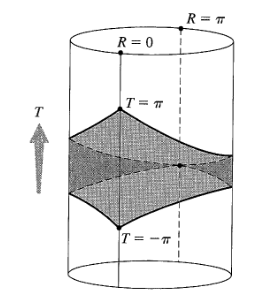
\includegraphics[width=.4\textwidth]{figures/ConfMink}
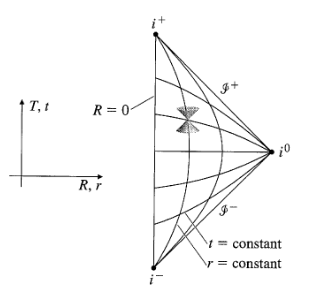
\includegraphics[width=.4\textwidth]{figures/confMink2}
\item On the above conformal diagram, label the following regions: future timelike infinity, spatial infinity, past timelike infinity, future null infinity, past null infinity. Which `infinity' do outgoing light rays end on? Which `infinity' to incoming light rays come from? 
\end{enumerate}





%
\end{document}